\documentclass[luatex,fontsize=8pt,paper=b5,twoside]{jlreq}%
\usepackage{amsmath,amssymb}
\usepackage{booktabs,caption}
\usepackage{luwa-ul, KKluaverb}
\usepackage[most]{tcolorbox}
\usepackage{luatexja-ruby}
\usepackage{KKran}

% You can omit these font settings.
\makeatletter
\RequirePackage[no-math]{fontspec}
\RequirePackage[no-math,match,scale=1]{luatexja-fontspec}
\RequirePackage[hiragino-pro,deluxe,expert]{luatexja-preset}
\setmainfont{HiraMinPro-W3}[BoldFont=HiraMinPro-W6]
\setmainjfont{HiraMinPro-W3}[BoldFont=HiraMinPro-W6]
\newfontfamily{\sfhira@pre}{HiraKakuPro-W3}[BoldFont=HiraKakuPro-W6]
\newjfontfamily{\sfhiraj@pre}{HiraKakuPro-W3}[BoldFont=HiraKakuPro-W6]
\newfontfamily{\mchira@pre}{HiraMinPro-W3}[BoldFont=HiraMinPro-W6]
\newjfontfamily{\mchiraj@pre}{HiraMinPro-W3}[BoldFont=HiraMinPro-W6]
\newfontfamily{\gthira@pre}{HiraKakuPro-W3}[BoldFont=HiraKakuPro-W6,FontFace={eb}{\shapedefault}{HiraKakuStd-W8}]
\newjfontfamily{\gthiraj@pre}{HiraKakuPro-W3}[BoldFont=HiraKakuPro-W6,FontFace={eb}{\shapedefault}{HiraKakuStd-W8}]
\newfontfamily{\mghira@pre}{HiraMaruPro-W4}
\newjfontfamily{\mghiraj@pre}{HiraMaruPro-W4}
\renewcommand{\sffamily}{\sfhira@pre\sfhiraj@pre}
\renewcommand{\mcfamily}{\mchira@pre\mchiraj@pre}
\renewcommand{\gtfamily}{\gthira@pre\gthiraj@pre}
\renewcommand{\mgfamily}{\mghira@pre\mghiraj@pre}
\makeatother
%%%


\usepackage{hyperref} 
\hypersetup{
  luatex, pdfencoding=auto, 
  colorlinks=true,
  linkcolor=black,     
  citecolor=black,     
  urlcolor=DeepSkyBlue3,      
  pdfborder={0 0 0}, 
}

\colorlet{grayLight}{white!80!black} 

\NewTCBListing{SourceCode}{ m m !o !O{DeepSkyBlue3} }{%
  enhanced, colback=black!70, colframe=Snow4,
  toptitle=-1mm, bottomtitle=-1mm,
  righttitle=-1mm, lefttitle=-1mm,
  arc=.5mm, 
  title={\tcbox[on line, arc=.5mm, boxsep=0pt, boxrule=0pt, top=1mm, bottom=0.8mm, left=2mm, right=2.2mm, colback=gray!80, coltext=white]{\raisebox{-0.1ex}{\vphantom{羅}\vphantom{j}#1}}},fonttitle=\gtfamily\footnotesize,boxrule=0.8pt,
  breakable,before upper={\color{white}},top=-0.5mm,bottom=-0.5mm,
  after title=\IfNoValueTF{#3}{}{{\hfill\tcbox[on line, arc=.5mm, boxsep=0pt, boxrule=0pt, top=1mm, bottom=0.8mm, left=2mm, right=2.2mm, colback=white!80!black, coltext=#4]{\raisebox{-0.1ex}{\vphantom{羅}\vphantom{j}#3}}}},
  listing only,
  listing options={
    language={#2},
    basicstyle=\ttfamily,
    keywordstyle=\ttfamily\color{white},
    stringstyle=\itshape\color{white},
    commentstyle=\small\gtfamily\color{DeepSkyBlue2},
    showspaces=false,showtabs=false,
    breaklines=true,breakindent=0pt,
    showstringspaces=false,
    columns=fullflexible,
    tabsize=2,
    numbers=left,numbersep=1.5pt,
    numberstyle=\scriptsize\gtfamily\color{gray},
  }
}

\NewTColorBox{OutPut}{ m !o !O{DeepSkyBlue3} }{%
  enhanced, colframe=Snow4,
  toptitle=-1mm, bottomtitle=-1mm,
  righttitle=-1mm, lefttitle=-1mm,
  arc=.5mm, colback=white, 
  title={\tcbox[on line, arc=.5mm, boxsep=0pt, boxrule=0pt, top=1mm, bottom=0.8mm, left=2mm, right=2.2mm, colback=gray!40, coltext=DeepSkyBlue3]{\raisebox{-0.1ex}{\vphantom{羅}\vphantom{j}#1}}},fonttitle=\gtfamily\footnotesize,boxrule=0.8pt,
  breakable,top=-0.5mm,bottom=-0.5mm,
  after title=\IfNoValueTF{#2}{}{{\hfill\tcbox[on line, arc=.5mm, boxsep=0pt, boxrule=0pt, top=1mm, bottom=0.8mm, left=2mm, right=2.2mm, colback=white!80!black, coltext=#3]{\raisebox{-0.1ex}{\vphantom{羅}\vphantom{j}#2}}}}, bottom=2mm, top=2mm, 
}

\title{\texttt{KKran} Package Documentation}
\author{Kosei Kawaguchi a.k.a. KKTeX}
\date{Version 1.1.6 (2026/02/20)}

\begin{document}
\begin{titlepage}
  \maketitle
\end{titlepage}
\newpage
\tableofcontents
\newpage

\section{Outline in English}
This is a package that offers commands for generating answer fields used in tests and exams. It is compatible with both vertical and horizontal text formatting. Using Lua and tikz, I made it possible to generate answer-boxes very easily. By the way, the naming may seem a bit odd, but the package name comes from ``欄 (ran)'' meaning ``a small space.'' I hope this package will be helpful to you.

\section{はじめに}
このパッケージは、オーソドックスなフォーマットの解答欄を作成するためのコマンドを提供するパッケージです。横書きと縦書きの両方に対応しています。内部的にLuaの構文を使用しているので、\namiKK{LuaLaTeX限定}です。

本パッケージによって、以下のような解答欄を作成することが可能です。サンプルのソースコードは本マニュアル末のセクションにあります。

\begin{center}
  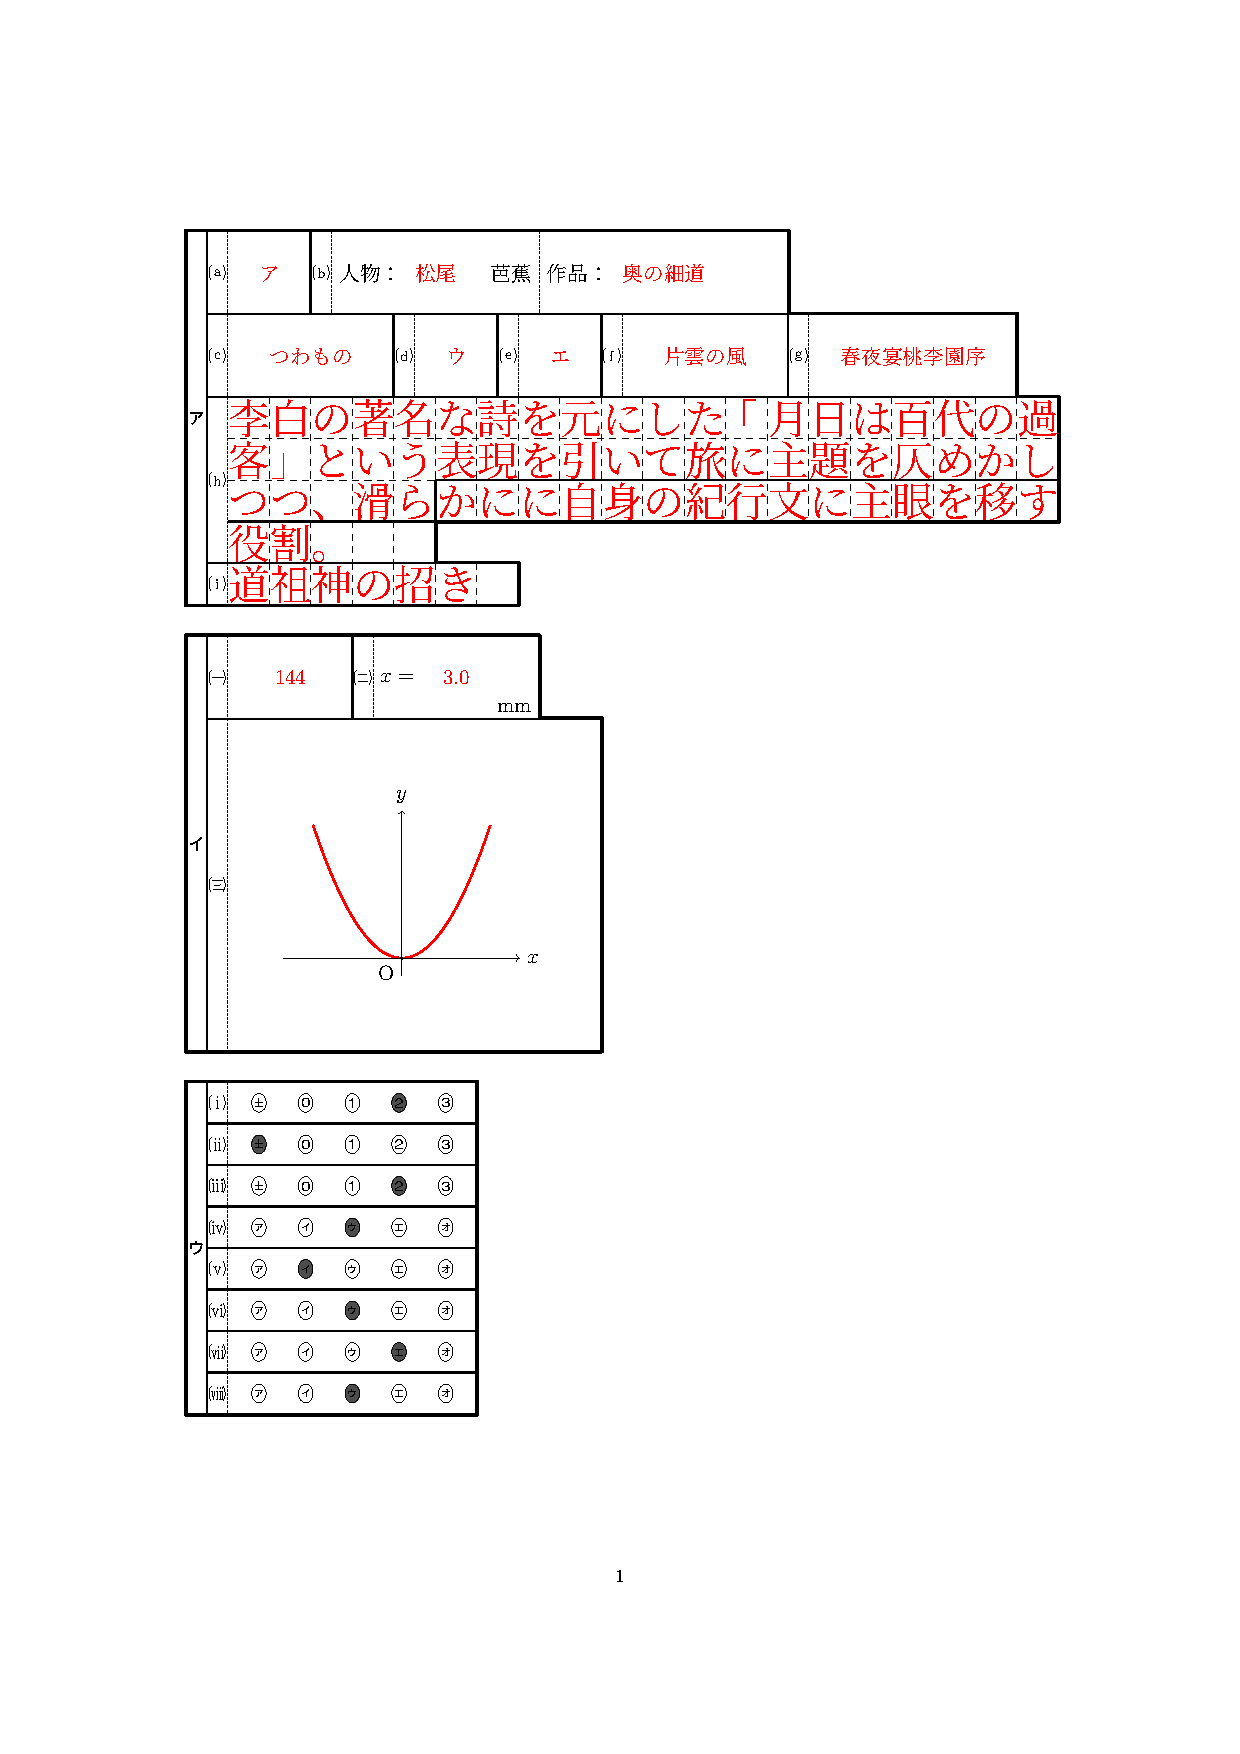
\includegraphics[width=.9\columnwidth]{kkran-sample.pdf}
\end{center}

\section{依存性}
内部的に読み込むパッケージは
\begin{itemize}\ttfamily
  \item calc, tikz
  \item xcolor, KKsymbols
  \item kvoptions, luacode
\end{itemize}
\noindent となります。

\section{設置・オプション}
しかるべき場所に\texttt{KKran.sty}が置かれている下で、\verb|\usepackage[オプション]{KKran}|により読み込みます。

パッケージオプションは

\begin{description}
  \item[\KKverb|kaitouhyouji|] 解答欄上に模範解答を出力するか否かを指定します。"0"なら出力せず、"1"なら出力します。デフォルトは１です。
  \item[\KKverb|kaitoucolor|] 模範解答の文字の色を指定します。デフォルトはredです。
  \item[\KKverb|gridmax|] マス目を出力するコマンドである\verb|\小問マス目| において、１行当たりの最大マス目数を指定します。デフォルトは20です。
  \item[\KKverb|nongridmax|] 記述解答欄を出力するコマンドである\verb|\小問記述| において、１行当たりの最大マス目数を指定します。ただし、このコマンドではマス目は可視化されません。デフォルトは20です。
  \item[\KKverb|unit|] 本パッケージでは「マス目単位で」各解答欄の位置を制御します。その際の１マスの幅を指定するのがこのオプションです。デフォルトは\verb|2\zw|です。
  \item[\KKverb|wakuwidth|] 解答欄の枠線の太さを指定します。デフォルトは\verb|.7pt|です。
  \item[\KKverb|tensenwakuwidth|] 欄の一部に使われている点線部分の太さを指定します。デフォルトは\verb|.7pt|です。
  \item[\KKverb|tensenon|] 欄の一部に使われている点線部分のdash-patternを決めるためのもので、線の最小単位の長さを指定できます。デフォルトは\verb|1pt|です。
  \item[\KKverb|tensenoff|] 欄の一部に使われている点線部分のdash-patternを決めるためのもので、最小単位の配置間隔を指定できます。デフォルトは\verb|1pt|です。
  \item[\KKverb|clsadjust|] jlreqクラス以外を指定する場合は、\verb|clsadjust=1|を指定します。一部クラスにおいて\verb|\小問マス目|に解答を入力した際、字間の調整が適切になされない事例があるためです。この値のデフォルトは0になっています。このオプションは内部的に、\verb|clsadjust=1|のとき
  \KKcodeS+
    \RequirePackage[scale=1]{luatexja-fontspec}
    \RequirePackage[deluxe,expert]{luatexja-preset}
  \KKcodeE
  \noindent を読み込むという処理をしています。したがって、より詳細にこれらのオプションを設定したい場合には\verb|clsadjust=0|とし、適宜設定をしてください。
  \item[\KKverb|fontdaimonbangou/fontshoumonbangou|] 大問番号／小問番号のフォントを\verb|\gtfamily|や\verb|\small|のような形式で指定します。デフォルトは\verb|\relax|（つまり指定なし）です。
  \item[\KKverb|styledaimonbangou/styleshoumonbangou|] 大問番号／小問番号のスタイルを指定します。指定するのは「制御綴名」です。例えば``\verb|\maru{引数}|''（\verb|KKsymbols|パッケージが提供）を使用して大問番号を丸数字にしたいという場合、\verb|styleshoumonbangou=maru|とします。デフォルトは\verb|kakko|となっています。特に括弧や丸などをつけたくない場合、\verb|全角幅固定|と指定するのが推奨されます。
\end{description}

\section{使い方}
\subsection{\KKverb|\KKran|}
このパッケージを使って解答欄を出力する場合、解答欄は\verb|\KKran[オプション]{引数}|の\verb|{引数}|に入れていくという形をとります。

\begin{SourceCode}{Input}{TeX}
  \KKran[解答欄の外枠を囲む線の太さ]{引数}[ナンバリングのオプション]
\end{SourceCode}

\noindent という構文です。

ナンバリングのオプションとは、番号をどの形式で進めるかを指定するもので、

\begin{SourceCode}{Input}{TeX}
  \KKran[解答欄の外枠を囲む線の太さ]{引数}[%
    daimon=いろは, shoumon=一
  ]
\end{SourceCode}

\noindent のような書き方をします。それぞれ何も指定しない場合は、アラビア数字でカウントされますが、そうでないカウント方法を取りたい場合、以下の選択肢から選ぶことになります。

\begin{description}
  \item[\KKverb|daimon|] a, A, あ, ア, いろは, イロハ, 一, ロ小, ロ大を取れる。それぞれ、abc\dots, ABC\dots, あいう\dots, アイウ\dots, いろは\dots, イロハ\dots, 一二三\dots, \Rrnum{1} \ \Rrnum{2} \ \Rrnum{3}\dots, \Rrnum*{1} \ \Rrnum*{2} \ \Rrnum*{3}\dots というカウント形式です。
  \item[\KKverb|shoumon|] 上に同じです。
\end{description}

\subsection{小問}
小問を構成する際は、\verb|\小問番号|で番号を、\verb|\小問欄|と\verb|\小問中欄|で欄をつけるという形です。

\begin{SourceCode}{Input}{TeX}
  % 構文
  \小問番号[横幅]{縦幅}[番号]
  % デフォルト
  % 横幅：.5
  % 番号：アラビア数字（\kakkoに入っている）

  % 使用例
  \KKran{%
    \小問番号[1]{2}\小問番号{2}[A]\小問番号{2}[B]\小問番号[1]{2}\小問番号[1]{2}
  }
\end{SourceCode}

\noindent が基本構文です。

出力は

\begin{OutPut}{Output}
  \KKran{%
    \小問番号[1]{2}\小問番号{2}[A]\小問番号{2}[B]\小問番号[1]{2}\小問番号[1]{2}
  }
\end{OutPut}

\noindent のようになります。

第３引数を指定しない場合、小問番号のカウンタは自動で進みますが、ここを手動で書いた場合はカウンタが進みません。
カウンタを強制的にある値にしたい場合には、\verb|\SetShoumon{99}|のように変更できるようにしてあります。

また、当然ながら大問が変わると値はリセットされます（大問の分け方は後述）。

ここに、\verb|\小問欄|および\verb|小問中欄|を組み合わせます。

\begin{SourceCode}{Input}{TeX}
  % 構文
  \小問欄{横幅}{縦幅}[欄内記入]
  \小問中欄{横幅}{縦幅}[欄内記入]
  % デフォルト
  % 欄内記入：空集合

  % 使用例
  \KKran{%
    \小問番号{2}\小問中欄{3}{2}\小問中欄{3}{2}\小問欄{4}{2}[south east={$\mathrm{mm}$}, west={$x=$}]\小問番号{2}\小問欄{4}{2}
  }
\end{SourceCode}

\begin{OutPut}{Output}
  \KKran{%
    \小問番号{2}\小問中欄{3}{2}\小問中欄{3}{2}\小問欄{4}{2}[south east={$\mathrm{mm}$}, west={$x=$}]\小問番号{2}\小問欄{4}{2}
  }
\end{OutPut}

基本的には\verb|\小問欄|を使いますが、同一の小問内で複数解答欄を用意する時などは、最後の欄以外を\verb|\小問中欄|にしても良いでしょう。

欄内記入に関して、オプションとして\KKverb|center,east,west,north east, north west, south east, south west|をとることができ、各key名に対応する箇所をアンカーポイントとしてその引数が出力されます。tikzにおけるnodeのオプションと全く同様です。

引数には何を挿入してもよく、図表も挿入可能です。

\begin{SourceCode}{Input}{TeX}
  \KKran{
    \小問番号{6}\小問欄{8}{6}[center={%
      \begin{tabular}{|l|c|r|}
      \hline
      列1 & 列2 & 列3 \\ \hline
      データA & 100 & 5.5 \\ \hline
      データB & 200 & 9.8 \\ \hline
      データC & 300 & 12.3 \\ \hline
      \end{tabular}
    }] 
    \小問番号{6}\小問欄{9}{6}[center={%
      \begin{tikzpicture}
        \draw[->] (0, -.3) -- (0, 2.5) node[above] {$y$};
        \draw[->] (-2, 0) -- (2, 0) node[right] {$x$};
        \filldraw (0, 0) circle (.5pt) node[below left] {$\mathrm{O}$};
        \draw[domain=-1.5:1.5, samples=100, thick] plot (\x, {\x*\x});
      \end{tikzpicture}
    }] 
  }
\end{SourceCode}

\begin{OutPut}{Output}
  \KKran{
    \小問番号{6}\小問欄{8}{6}[center={%
      \begin{tabular}{|l|c|r|}
      \hline
      列1 & 列2 & 列3 \\ \hline
      データA & 100 & 5.5 \\ \hline
      データB & 200 & 9.8 \\ \hline
      データC & 300 & 12.3 \\ \hline
      \end{tabular}
    }] 
    \小問番号{6}\小問欄{9}{6}[center={%
      \begin{tikzpicture}
        \draw[->] (0, -.3) -- (0, 2.5) node[above] {$y$};
        \draw[->] (-2, 0) -- (2, 0) node[right] {$x$};
        \filldraw (0, 0) circle (.5pt) node[below left] {$\mathrm{O}$};
        \draw[domain=-1.5:1.5, samples=100, thick] plot (\x, {\x*\x});
      \end{tikzpicture}
    }] 
  }
\end{OutPut}

\subsection{模範解答入力}
模範解答を入力する場合、その部分を\verb|\KaitouInput{引数}|によって入力しておくと、パッケージオプションである\texttt{kaitouhyouji}が1の時だけ表示されるようになります。ただし、この効果は\verb|\color|コマンドによる色の変更が可能な範囲に限ります。

tikzの描画も当然解答として入力可能ですが、

\begin{SourceCode}{Input}{TeX}
  \KKran{
    \小問番号{6}\小問欄{9}{6}[center={\KaitouInput{%
      \begin{tikzpicture}
        \draw[->] (0, -.3) -- (0, 2.5) node[above] {$y$};
        \draw[->] (-2, 0) -- (2, 0) node[right] {$x$};
        \filldraw (0, 0) circle (.5pt) node[below left] {$\mathrm{O}$};
        \draw[domain=-1.5:1.5, samples=100, thick, blue] plot (\x, {\x*\x}); % ここ！
      \end{tikzpicture}
    }}] 
  }
\end{SourceCode}

\begin{OutPut}{Output}
    \KKran{
    \小問番号{6}\小問欄{9}{6}[center={\KaitouInput{%
      \begin{tikzpicture}
        \draw[->] (0, -.3) -- (0, 2.5) node[above] {$y$};
        \draw[->] (-2, 0) -- (2, 0) node[right] {$x$};
        \filldraw (0, 0) circle (.5pt) node[below left] {$\mathrm{O}$};
        \draw[domain=-1.5:1.5, samples=100, thick, blue] plot (\x, {\x*\x}); % ここ！
      \end{tikzpicture}
    }}] 
  }
\end{OutPut}

のように明示的に色を指定した場合、そこだけは\verb|\KaitouInput|の効果範囲外となることに注意しましょう。

\section{大問ごとの組み方}
大問を組むとなる場合、\verb|\大問番号|というコマンドで番号をつけ、段ごとに\verb|\小問欄|などを並べていきます。段をずらす際には\verb|\GoDown|というコマンドを使用していきます。

\begin{SourceCode}{Input}{TeX}
  % 構文
  \大問番号[横幅]{縦幅}[番号]
  % デフォルト
  % 横幅：.5
  % 番号：アラビア数字（\kakkoに入っている）

  \GoDown{下に降りたいマス目数}

  % 使用例
  \KKran[3pt]{%
    \大問番号[1]{9}
    \小問番号{2}\小問欄{2}{2}\小問番号{2}\小問欄{4}{2}\GoDown{2}
    \小問番号{4}\小問欄{8}{4}\GoDown{4}
    \小問番号{3}\小問欄{3}{3}\小問番号{3}\小問欄{2}{3}
  }[shoumon=いろは,daimon=ア]
\end{SourceCode}

\begin{OutPut}{Output}
  \KKran[3pt]{%
    \大問番号[1]{9}
    \小問番号{2}\小問欄{2}{2}\小問番号{2}\小問欄{4}{2}\GoDown{2}
    \小問番号{4}\小問欄{8}{4}\GoDown{4}
    \小問番号{3}\小問欄{3}{3}\小問番号{3}\小問欄{2}{3}
  }[shoumon=いろは,daimon=ア]
\end{OutPut}

大問番号をある値にしたいという場合、\verb|\SetDaimon{99}|のように指定します。

\section{記述解答欄}
記述問題専用の解答欄として、マス目ありのもの、なしのものの２種類の解答欄を用意しています。

注意点として、\verb|\linewidth|を上回る横幅を解答欄が占めるような組み方をしてはならないというものがあります。エラーにはなりませんが、大問と大問との間隔が余計に１行分大きくなってしまいます。

\begin{SourceCode}{Input}{TeX}
  % 構文
  \小問マス目[文字数下限]{文字数上限}[欄内記入]
  \小問記述{文字数上限}[欄内記入]
  % デフォルト
  % 文字数下限：文字数上限と同じ値
  % 欄内記入：空集合

  % 使用例
  \KKran[3pt]{%
    \大問番号[1]{7}
    \小問番号{1}\小問マス目[4]{6}\GoDown{1}
    \小問番号{2}\小問記述{40}\GoDown{2}
    \小問番号{4}\小問マス目[50]{75}
  }
\end{SourceCode}

\begin{OutPut}{Output}
  \KKran[3pt]{%
    \大問番号[1]{7}
    \小問番号{1}\小問マス目[4]{6}\GoDown{1}
    \小問番号{2}\小問記述{40}\GoDown{2}
    \小問番号{4}\小問マス目[50]{75}
  }
\end{OutPut}

また、ここに模範解答を入力する際は半角英数字や約物を全角１マスに適切に拡大縮小するため、必要に応じて\verb|\全角幅固定|というコマンドを使用します。

\begin{SourceCode}{Input}{TeX}
  % 使用例
  \KKran[3pt]{%
    \大問番号[1]{3}
    \小問番号{1}\小問マス目[4]{6}[\KaitouInput{\全角幅固定{12}\全角幅固定{3}番目\全角幅固定{。}}]\GoDown{1}
    \小問番号{2}\小問マス目{40}[\KaitouInput{\全角幅固定{「}日本に\全角幅固定{Ma}\全角幅固定{tt}\全角幅固定{he}\全角幅固定{w\phantom{w}}＝\全角幅固定{Pe}\全角幅固定{rr}\全角幅固定{y\phantom{y}}提督が来たから。\全角幅固定{」}という話であります。}]
  }
\end{SourceCode}

\begin{OutPut}{Output}
  \KKran[3pt]{%
    \大問番号[1]{3}
    \小問番号{1}\小問マス目[4]{6}[\KaitouInput{\全角幅固定{12}\全角幅固定{3}番目\全角幅固定{。}}]\GoDown{1}
    \小問番号{2}\小問マス目{40}[\KaitouInput{\全角幅固定{「}日本に\全角幅固定{Ma}\全角幅固定{tt}\全角幅固定{he}\全角幅固定{w\phantom{w}}＝\全角幅固定{Pe}\全角幅固定{rr}\全角幅固定{y\phantom{y}}提督が来たから。\全角幅固定{」}という話であります。}]
  }
\end{OutPut}

\section{マークシート}
マークシートの作り方は、\verb|\MarkArrayMake|でひとまず必要な配列を作成しておき、\verb|\マークシート|コマンドで配置します。この機能に関しては、横書きモードでのみ使用されることを想定していることに注意してください\footnote{縦書き環境に入っても出力が著しく乱れたりエラーになったりはしませんが、そもそもマークシートは横に楕円を並べるものであるため、縦書きの文書と併用する場合にはlltjextなどと併用し部分横書きを使うことを推奨します。}。

\begin{SourceCode}{Input}{TeX}
  % 構文
  \MarkArrayMake{配列名}{|要素1|要素2|...|要素n|}
  \マークシート{配置幅}{配列格納}[正解番号]

  % 使用例
  \MarkArrayMake{テストA}{|$\pm$|0|1|2|3|}
  \MarkArrayMake{テストB}{|ア|イ|ウ|エ|オ|}
  \KKran[3pt]{%
    \大問番号[1]{8}
    \小問番号{1}\小問欄{6}{1}[center=\マークシート{5}{\テストAマーク配列}[4]]\GoDown{1}
    \小問番号{1}\小問欄{6}{1}[center=\マークシート{5}{\テストAマーク配列}[1]]\GoDown{1}
    \小問番号{1}\小問欄{6}{1}[center=\マークシート{5}{\テストAマーク配列}[4]]\GoDown{1}
    \小問番号{1}\小問欄{6}{1}[center=\マークシート{5}{\テストBマーク配列}[3]]\GoDown{1}
    \小問番号{1}\小問欄{6}{1}[center=\マークシート{5}{\テストBマーク配列}[2]]\GoDown{1}
    \小問番号{1}\小問欄{6}{1}[center=\マークシート{5}{\テストBマーク配列}[3]]\GoDown{1}
    \小問番号{1}\小問欄{6}{1}[center=\マークシート{5}{\テストBマーク配列}[4]]\GoDown{1}
    \小問番号{1}\小問欄{6}{1}[center=\マークシート{5}{\テストBマーク配列}[3]]\GoDown{1}
  }[shoumon=一,daimon=ア]
\end{SourceCode}

\begin{OutPut}{Output}
  \MarkArrayMake{テストA}{|$\pm$|0|1|2|3|}
  \MarkArrayMake{テストB}{|ア|イ|ウ|エ|オ|}
  \KKran[3pt]{%
    \大問番号[1]{8}
    \小問番号{1}\小問欄{6}{1}[center=\マークシート{5}{\テストAマーク配列}[4]]\GoDown{1}
    \小問番号{1}\小問欄{6}{1}[center=\マークシート{5}{\テストAマーク配列}[1]]\GoDown{1}
    \小問番号{1}\小問欄{6}{1}[center=\マークシート{5}{\テストAマーク配列}[4]]\GoDown{1}
    \小問番号{1}\小問欄{6}{1}[center=\マークシート{5}{\テストBマーク配列}[3]]\GoDown{1}
    \小問番号{1}\小問欄{6}{1}[center=\マークシート{5}{\テストBマーク配列}[2]]\GoDown{1}
    \小問番号{1}\小問欄{6}{1}[center=\マークシート{5}{\テストBマーク配列}[3]]\GoDown{1}
    \小問番号{1}\小問欄{6}{1}[center=\マークシート{5}{\テストBマーク配列}[4]]\GoDown{1}
    \小問番号{1}\小問欄{6}{1}[center=\マークシート{5}{\テストBマーク配列}[3]]\GoDown{1}
  }[shoumon=一,daimon=ア]
\end{OutPut}

\verb|\マークシート{配置幅}{配列格納}[正解番号]|の第３引数で指定した番号を$n \in \mathbb{N}$として、作成した配列の$n$番目が黒く塗られる仕様となっており、模範解答の入力はこれで行います。\verb|kaitouhyouji=0|の時は塗られず、\verb|kaitouhyouji=1|のときにのみ黒く塗った部分が表示されます。

\section{サンプル}
\begin{SourceCode}{Input}{TeX}
  \documentclass[paper=a4]{jlreq}

  \usepackage[
    kaitouhyouji=1,
    gridmax=20,
    kaitoucolor=red,
    fontdaimonbangou=\gtfamily,
    styledaimonbangou=全角幅固定
  ]{KKran}

  \begin{document}
  \KKran{%
    \大問番号{9}
    \小問番号{2}\小問欄{2}{2}[center=\KaitouInput{ア}]\小問番号{2}\小問中欄{5}{2}[west=人物：,center=\KaitouInput{松尾},east=芭蕉]\小問欄{6}{2}[west=作品：,center=\KaitouInput{奥の細道}]\GoDown{2}
    \小問番号{2}\小問欄{4}{2}[center=\KaitouInput{つわもの}]\小問番号{2}\小問欄{2}{2}[center=\KaitouInput{ウ}]\小問番号{2}\小問欄{2}{2}[center=\KaitouInput{エ}]
    \小問番号{2}\小問欄{4}{2}[center=\KaitouInput{片雲の風}]
    \小問番号{2}\小問欄{5}{2}[center=\KaitouInput{春夜宴桃李園序}]\GoDown{2}
    \小問番号{4}\小問マス目[45]{65}[\KaitouInput{李白の著名な詩を元にした\全角幅固定{「}月日は百代の過客\全角幅固定{」}という表現を引いて旅に主題を仄めかしつつ\全角幅固定{、}滑らかにに自身の紀行文に主眼を移す役割\全角幅固定{。}}]\GoDown{4}
    \小問番号{1}\小問マス目{7}[\KaitouInput{道祖神の招き}]
  }[shoumon=a,daimon=ア]
  \bigskip

  \KKran{%
    \大問番号{10}\小問番号{2}\小問欄{3}{2}[center=\KaitouInput{144}]\小問番号{2}\小問欄{4}{2}[south east={$\mathrm{mm}$},center=\KaitouInput{$3.0$}, west={$x=$}]\GoDown{2}
    \小問番号{8}\小問欄{9}{8}[center={\KaitouInput{%
      \begin{tikzpicture}
        \draw[domain=-1.5:1.5, samples=100, thick] plot (\x, {\x*\x});
        \draw[->,, black] (0, -.3) -- (0, 2.5) node[above] {$y$};
        \draw[->,, black] (-2, 0) -- (2, 0) node[right] {$x$};
        \filldraw[black] (0, 0) circle (.5pt) node[below left] {$\mathrm{O}$};
      \end{tikzpicture}}}]
  }[shoumon=一,daimon=ア]
  \bigskip

  \MarkArrayMake{テストA}{|$\pm$|0|1|2|3|}
  \MarkArrayMake{テストB}{|ア|イ|ウ|エ|オ|}
  \KKran{%
    \大問番号{8}
    \小問番号{1}\小問欄{6}{1}[center=\マークシート{5}{\テストAマーク配列}[4]]\GoDown{1}
    \小問番号{1}\小問欄{6}{1}[center=\マークシート{5}{\テストAマーク配列}[1]]\GoDown{1}
    \小問番号{1}\小問欄{6}{1}[center=\マークシート{5}{\テストAマーク配列}[4]]\GoDown{1}
    \小問番号{1}\小問欄{6}{1}[center=\マークシート{5}{\テストBマーク配列}[3]]\GoDown{1}
    \小問番号{1}\小問欄{6}{1}[center=\マークシート{5}{\テストBマーク配列}[2]]\GoDown{1}
    \小問番号{1}\小問欄{6}{1}[center=\マークシート{5}{\テストBマーク配列}[3]]\GoDown{1}
    \小問番号{1}\小問欄{6}{1}[center=\マークシート{5}{\テストBマーク配列}[4]]\GoDown{1}
    \小問番号{1}\小問欄{6}{1}[center=\マークシート{5}{\テストBマーク配列}[3]]\GoDown{1}
  }[shoumon=ロ小,daimon=ア]

  \end{document}
\end{SourceCode}

\begin{OutPut}{Output}
  \begin{center}
    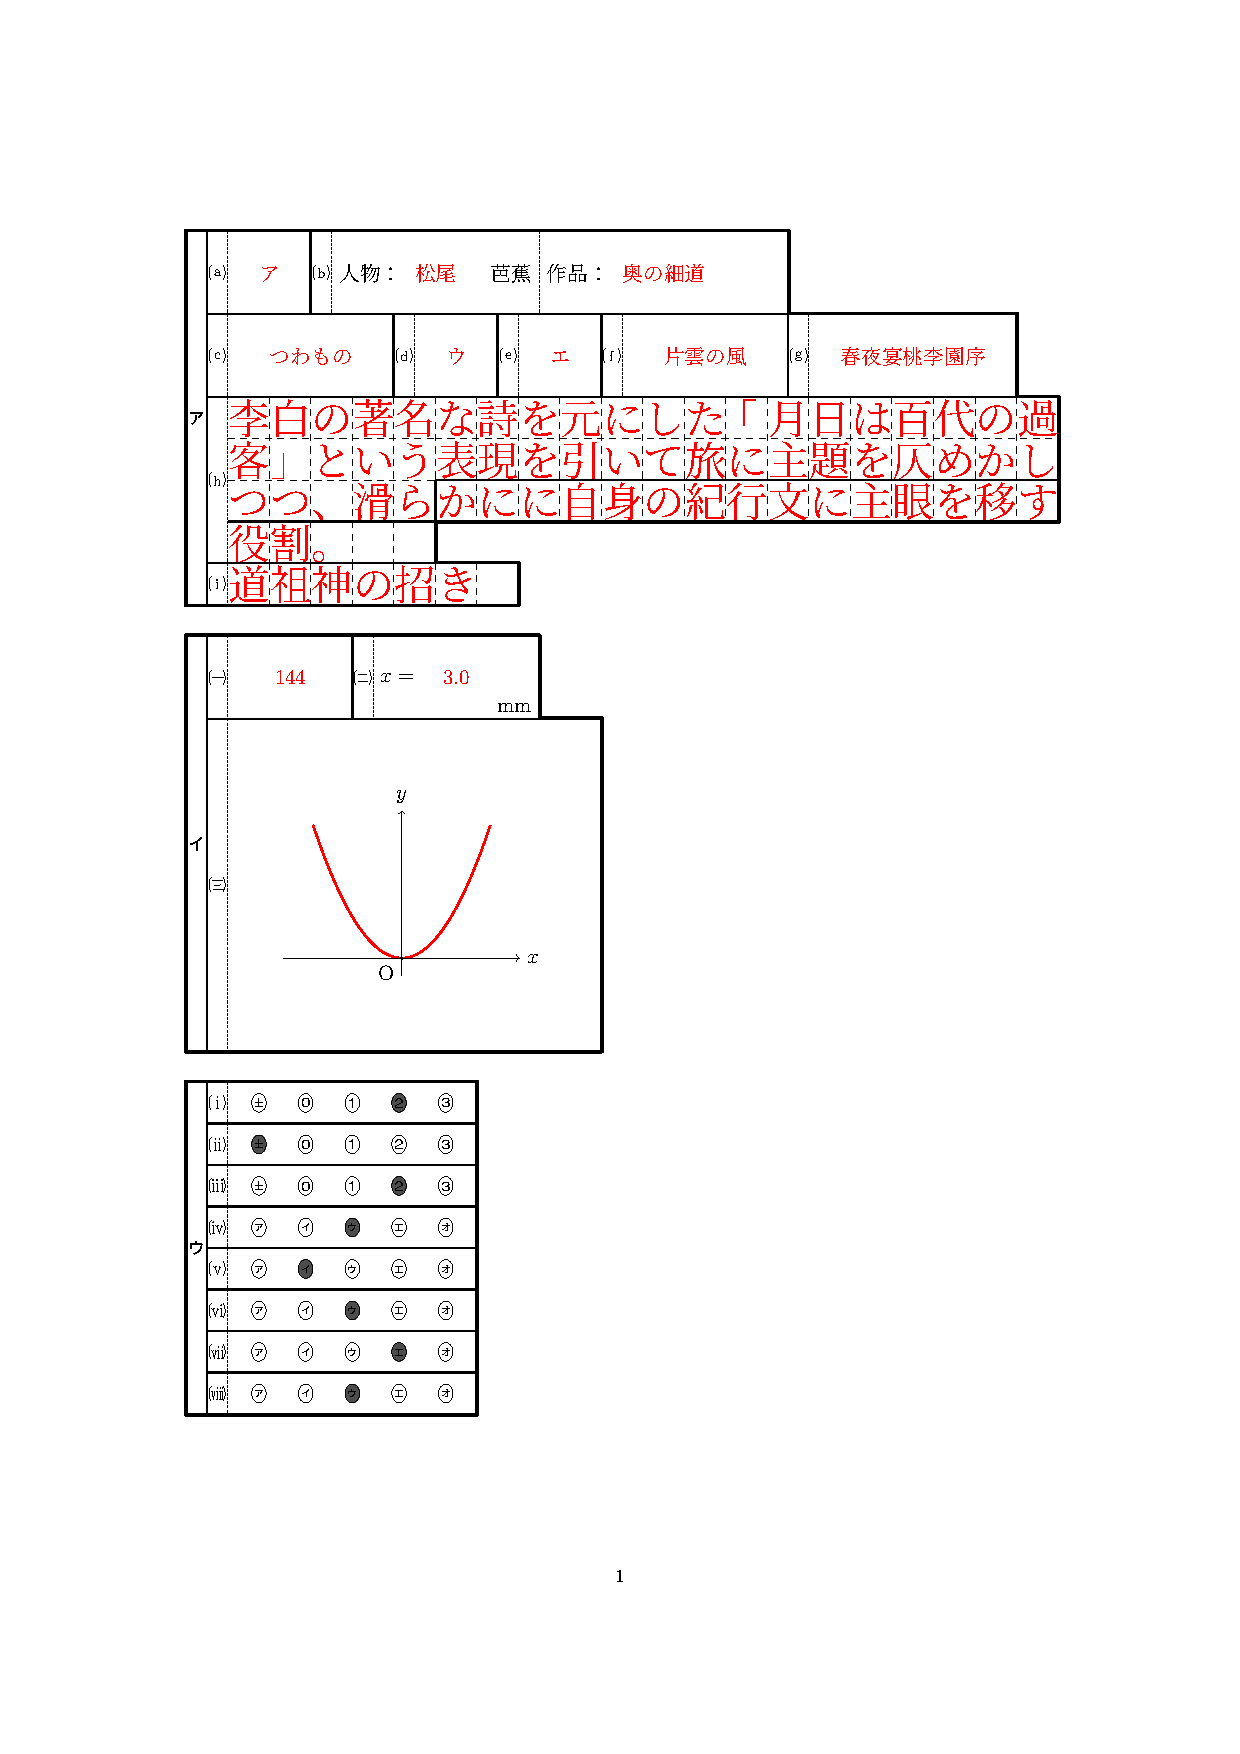
\includegraphics[width=.7\columnwidth]{kkran-sample.pdf}
  \end{center}
\end{OutPut}

\section{Version History}
\begin{itemize}
  \item \textbf{v1.0.0 (2025/11/23)} --- Initial public release.
  \item \textbf{v1.1.0 (2025/12/23)} --- Changed internal behavior in order to follow KKsymbols v2.0.0
  \item \textbf{v1.1.2 (2026/01/02)} --- Added license file and improved README file. In addition, the manual has been updated to reflect bug fixes introduced in luatexja version 20260107.0.
  \item \textbf{v1.1.4 (2026/02/15)} --- I changed the following points:
  \begin{itemize}
    \item Fixed a bug where the left border of \verb|\小問欄|, \verb|\小問中欄|, \verb|\小問マス目|, and \verb|\小問記述| produce unwanted thin line.
    \item Add some package options in order to set font and style of ``大問番号'' and ``小問番号''.
    \item Add a new command \verb|\全角幅固定| to input ``半角英数字'' to the optional argument of \verb|\小問マス目|.
    \item Changed some dafault values of package options.
  \end{itemize}
  \item \textbf{v1.1.5 (2026/02/17)} --- Fixed a bug where unwanted ``\KKverb|*|'' is output when \KKverb|styledaimon/shoumonbangou=全角幅固定| is specified and the optional argument of \KKverb|\KKran| is set as \KKverb|[shoumon=a]| or \KKverb|[daimon=a]|. 
  \item \textbf{v1.1.6 (2026/02/20)} --- Improved the output of the dashed lines of \KKverb|\小問マス目|. 
\end{itemize}

\end{document}